\subsection{Logic Layer}
\subsubsection{Overview}
The logic layer of the TAMP program functions as a Task Planner, managing the discrete portion of the search to find semantic solutions. These solutions are sequences of state configurations, each differing by one module movement, that transform the initial state configuration into the goal state configuration.
\\\\
While many contemporary task planners use machine learning techniques to find solutions, these are unsuitable for the space industry due to their black box behaviour. Instead, the TAMP program employs simple graph search techniques to ensure transparency and reliability.

\subsubsection{Searching the Graph}
To search the graph and find the path to the goal state configuration, two major search algorithms are considered: Depth-First Search (DFS) and Breadth-First Search (BFS).
\begin{itemize}[]
	\item\textbf{Depth-First Search (DFS):} In DFS, the algorithm explores a path to its full depth before backtracking and trying alternative paths. This can be implemented using a state priority queue that sorts states based on their proximity to the goal state, enabling quick solutions. However, the resulting path may not be the most efficient for the mobile manipulator, as each state transition involves additional movement.
	\item\textbf{Breadth-First Search (BFS):} In contrast, BFS explores all states at one depth level before proceeding to the next level. It searches all states one step away from the starting state, then two steps away, and so on. Although BFS is much slower than DFS and less scalable to larger numbers of modules, it guarantees finding paths with the fewest transitions to the goal state, making it more suitable for efficient reconfiguration.
\end{itemize}
Given the requirement for solution efficiency over planner speed, the Task Planner implements the BFS algorithm. The pseudo-code for the Task Planner algorithm is shown in Listing \ref{SearchPseudo}.

\begin{lstlisting}[caption={Task Planner search algorithm pseudo-code},captionpos=b,label={SearchPseudo}]
	FIND PATH (S_start, S_goal, max_branches)
	search_tree <- []
	S_current <- S_start
	WHILE S_current NOT S_goal DO
	PriorityQ <- GenNewStates(S_current)
	FOR max_branches DO
	S_new <- PriorityQ.pop(0)
	S_new.parent <- S_current
	search_tree.add(S_new)
	END	
	S_current <- search_tree.pop(0)
	END
	RETURN S_current.GetStatePath()
\end{lstlisting}

\subsubsection{Generating States}
To expand the graph, the task planner generates new states using the \textbf{'GenNewStates()'} function, referenced in the search algorithm pseudo-code (Listing \ref{SearchPseudo}). States are generated based on a set of rules that prioritize which modules to move, ensuring efficient state expansion. The priority rules for module movement are as follows:
\begin{enumerate}[]
	\item Modules not yet in their final position
	\item Modules adjacent to modules not yet in their final position
	\item Remaining modules 
\end{enumerate}
These rules ensure that the task planner consistently generates new states while prioritizing the movement of modules that need to be repositioned first. This approach minimizes unnecessary movements and helps streamline the reconfiguration process.
\\\\
A priority queue that prioritizes modules based on their distance from modules not yet in their final position was considered. This would allow for efficient repositioning of deeply embedded modules. However, this added complexity was deemed unnecessary for the current program's scope and would increase computation time for a relatively rare scenario. For larger structures, implementing such a priority queue could be beneficial to improve computation efficiency.

\subsubsection{Trimming States}
When handling inputs with large numbers of modules, the search tree expansion can quickly result in a vast number of states, consuming significant memory, and computation time. To expedite the search process, generated states are sorted into a priority queue, and only the highest priority states are added to the search graph. The remaining states are discarded, as illustrated in Figure \ref{treeTrimming}. The states are prioritized based on their proximity to the desired goal configuration, using the following heuristics:
\begin{itemize}[]
	\item Number of modules already in their final positions.
	\item Number of modules not in their final positions but occupying positions that are vacant in the goal state.
	\item Sum of the Euclidean distances of the module positions from their final positions in the goal state.
\end{itemize}
These heuristics measure how far a state is from the goal state and allow comparison between states to determine which is closer to the goal. States are first sorted using the number of modules in their final positions. In the event of a tie, the second heuristic is used. If there is still a tie, the computationally intensive third heuristic is applied.
\\\\
By primarily using the first two heuristics, the planner reduces the frequency of expensive calculations, thereby speeding up the state comparison process and improving overall efficiency.
\\\\
\begin{figure*}[h]
	\centering
	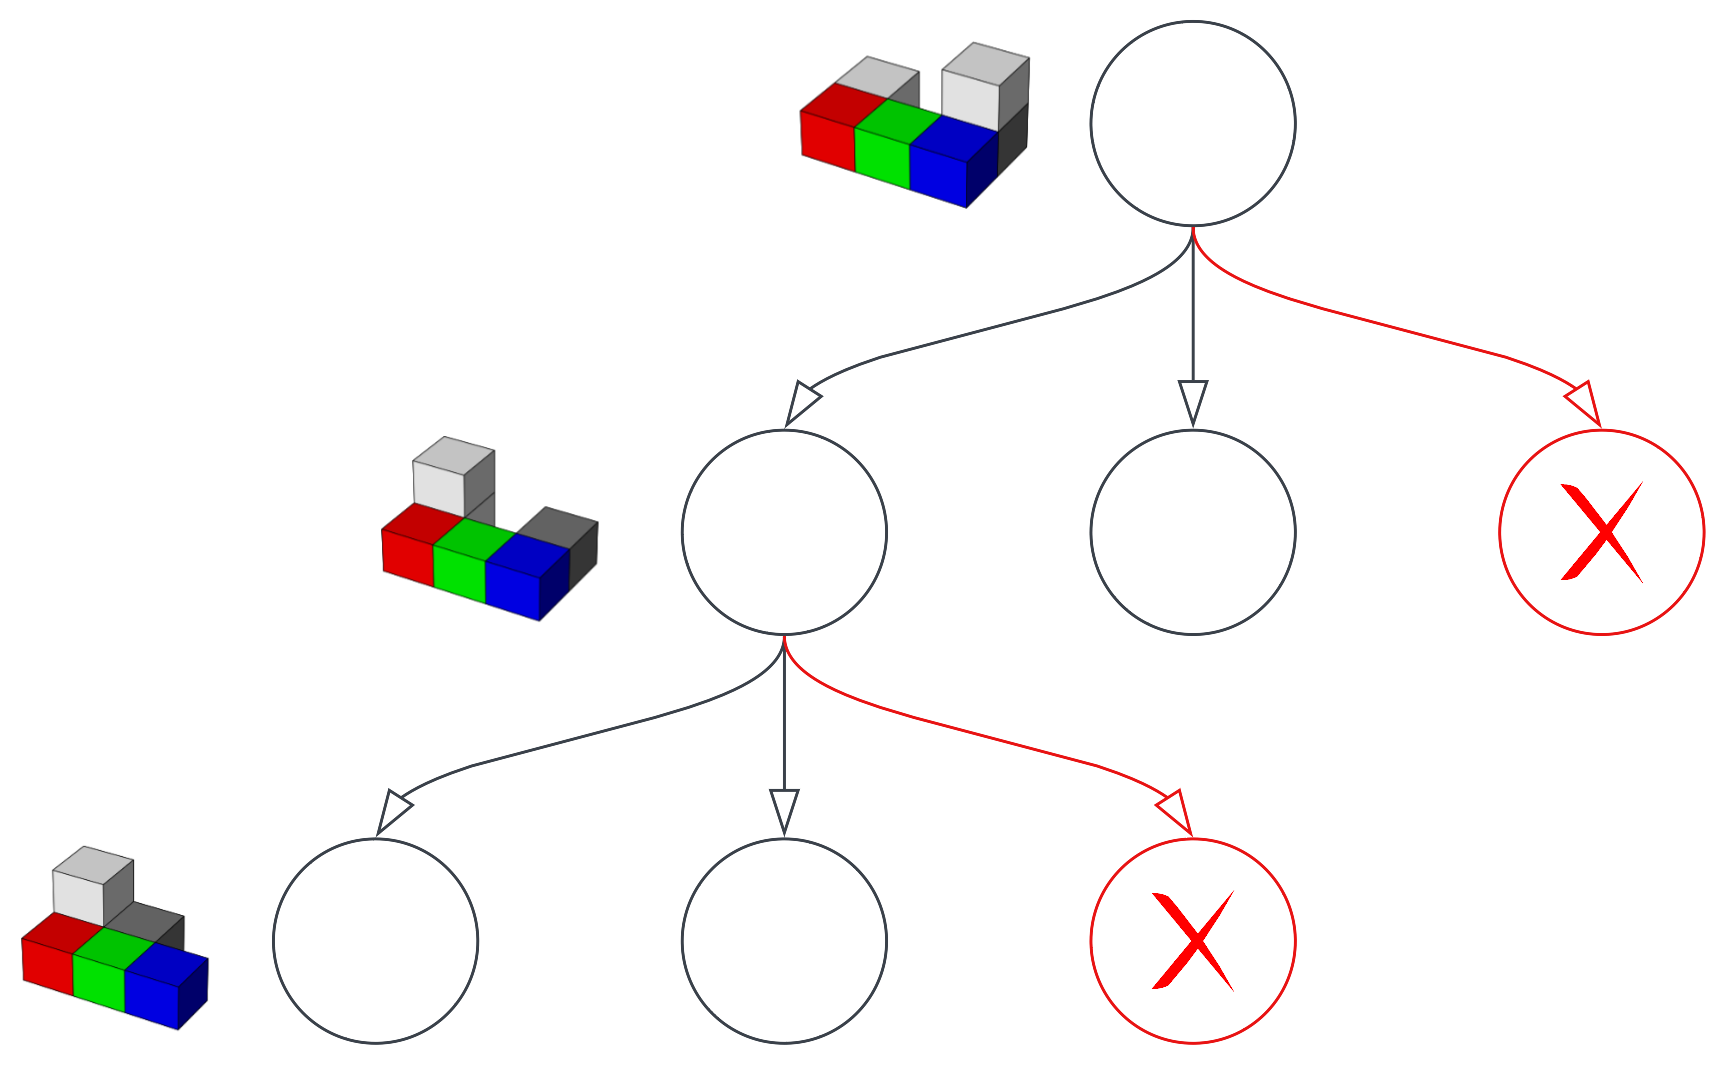
\includegraphics[width=0.7\textwidth]{treeTrimming.png}
	\caption{Selection of generated states demonstration}
	\label{treeTrimming}
\end{figure*}

\subsubsection{Physical Layer Feedback}
When a semantic solution is identified, it is passed to the physical layer for verification. If the physical layer encounters a failure, the transition causing the failure is pruned from the search tree, and all subsequent transitions on that branch are removed. The search then resumes without the failing transition.
\\\\
An alternative approach would involve performing physical layer checks for each move during state generation. However, physical layer calculations are significantly more computationally intensive compared to those in the logic layer. Thus, it is more efficient to focus on verifying only the transitions within the semantic solution, even if it means spending more time searching for these solutions. This approach balances computational load by leveraging the relatively quicker logic layer to identify potential solutions and reserving the intensive checks for validation.
